\chapter{Design}
This chapter contains the choices made regarding the process of
designing the front-end of the application, for a more technical
approach see \textit{System Architecture chapter 6}.

\section{Design process}
\label{sec:designProcess}

The user interface provided by the previous IDI Open system consisted of
a simple web interface for reading news items, registering teams for
contests, and delivering submissions. GentleIDI is intended to provide
more functionality through its web interface, including but not limited
to judge supervision(requirement FJ-11) and user management 
(requirements FC-01, FC-03 and FC-04). As a consequence
we had two options available: reusing and extending the existing
interface design, or creating our own design from scratch.

\begin{figure}[h!]
	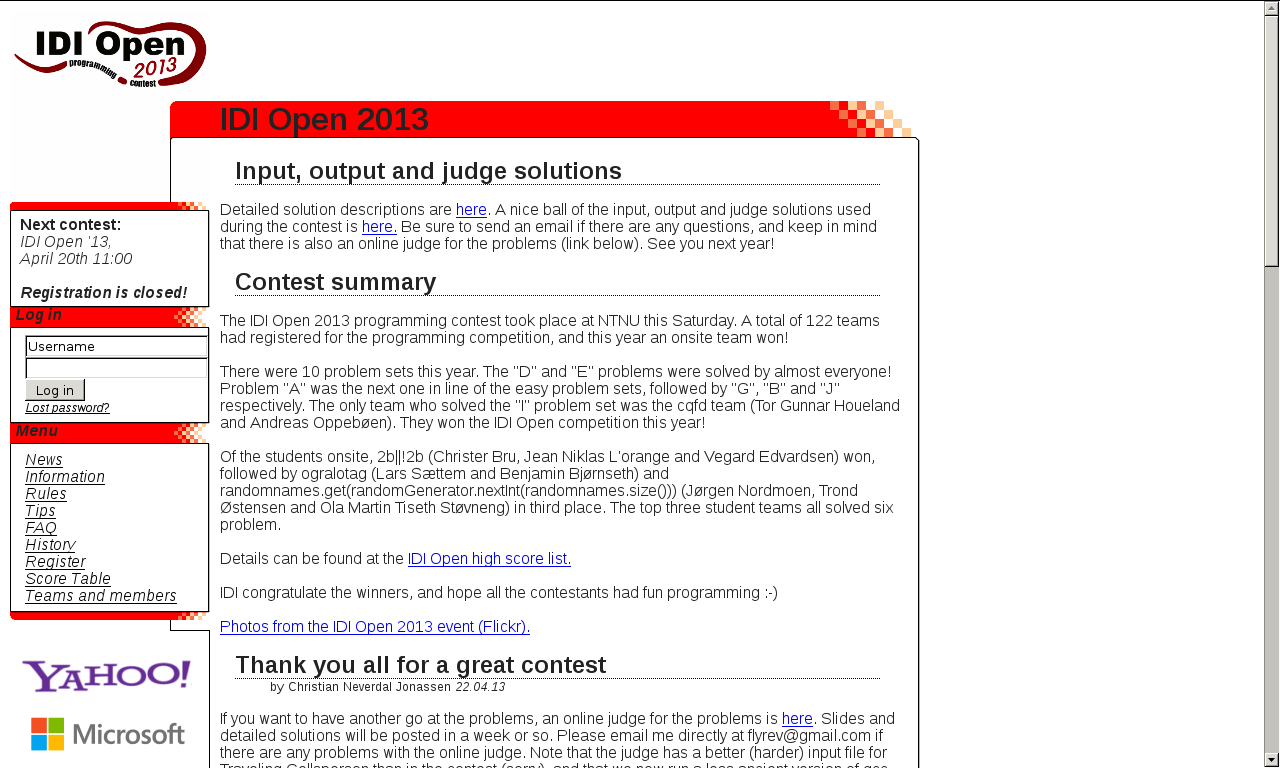
\includegraphics[width=6.278in,height=3.7638in]{a07Design-img1.png} 
	\caption{User Interface of the old system}
	\label{fig:oldSystem}
\end{figure}

We chose to create our own design from scratch, while still trying to
keep a similar placement of elements from the previous design. The
customer expressed concern regarding how contestants would react to the
transition from the old interface to the new one. With this in mind we
started to create mockups modelling core elements of the website. Our
initial drafts consisted of simple rearrangements of elements found in
the old web interface.

\begin{figure}[h!]
	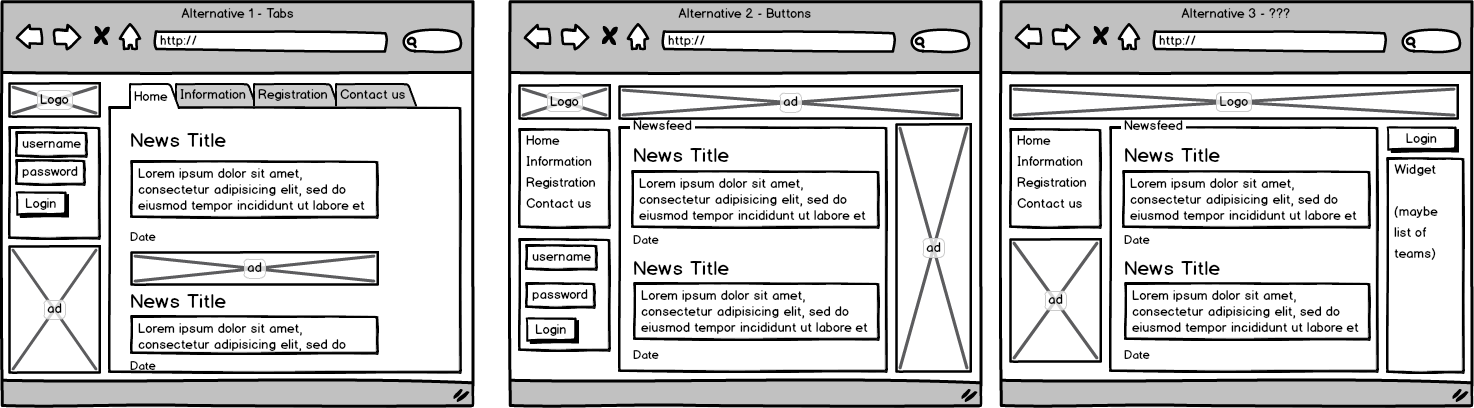
\includegraphics[width=6.278in,height=1.7362in]{a07Design-img2.png} 
	\caption{Initial mockups}
	\label{fig:mockup}
\end{figure}

Beyond our three initial mockups we tried a couple of ``out
of the box'' approaches to our designs, but none of them
met our standard and was rejected for either being too time-consuming
to implement or too far from what our customer wanted. We had a meeting
with our customer, where we showed our mockups, and what our thoughts
on design had been so far. We wanted to make sure that the customer
was on the same page as us, and that we were not moving beyond the
scope of the project. Our customer was not very focused
on the design aspect, but one demand they had was that they wanted the
new site to have the same structure as the old one. One example of what
this means is that the customer wanted us to keep the menu on the
left side as you can see that the old system has in Fig~\ref{fig:oldSystem}. We agreed,
because getting used to a new website can take time, so keeping the
structure similar would ease the transition for our users. With this in
mind we decided to go for one of our initial mockups, the rightmost one
in Fig~\ref{fig:mockup}, because it had the same structure as the old page, and we
personally favoured that design. As a result, most of the elements
found in the old interface can be found in the new one, and the
transition between using the two is reduced to a minimum.

The task had to be completed in time for milestone M-03, so our main
concern was designing for the functionality needed for that particular
milestone. However, we also had mockups for functionality outside of
this milestone. After milestone M-03 was met, we introduced new designs
for new functionality through continuous work on top of a template.

The majority of the front end is stylized using bootstrap[Link til
kilde] as a framework, enabling us to create a site which is both
highly maintainable and aesthetically pleasing at the same time. The
admin interface was created using django-admin-interface. Grappelli
was used as a skin to give it a modern look. The look of the final page
can be viewed in Fig~\ref{fig:finalUI}.


 \begin{figure}[h!]
	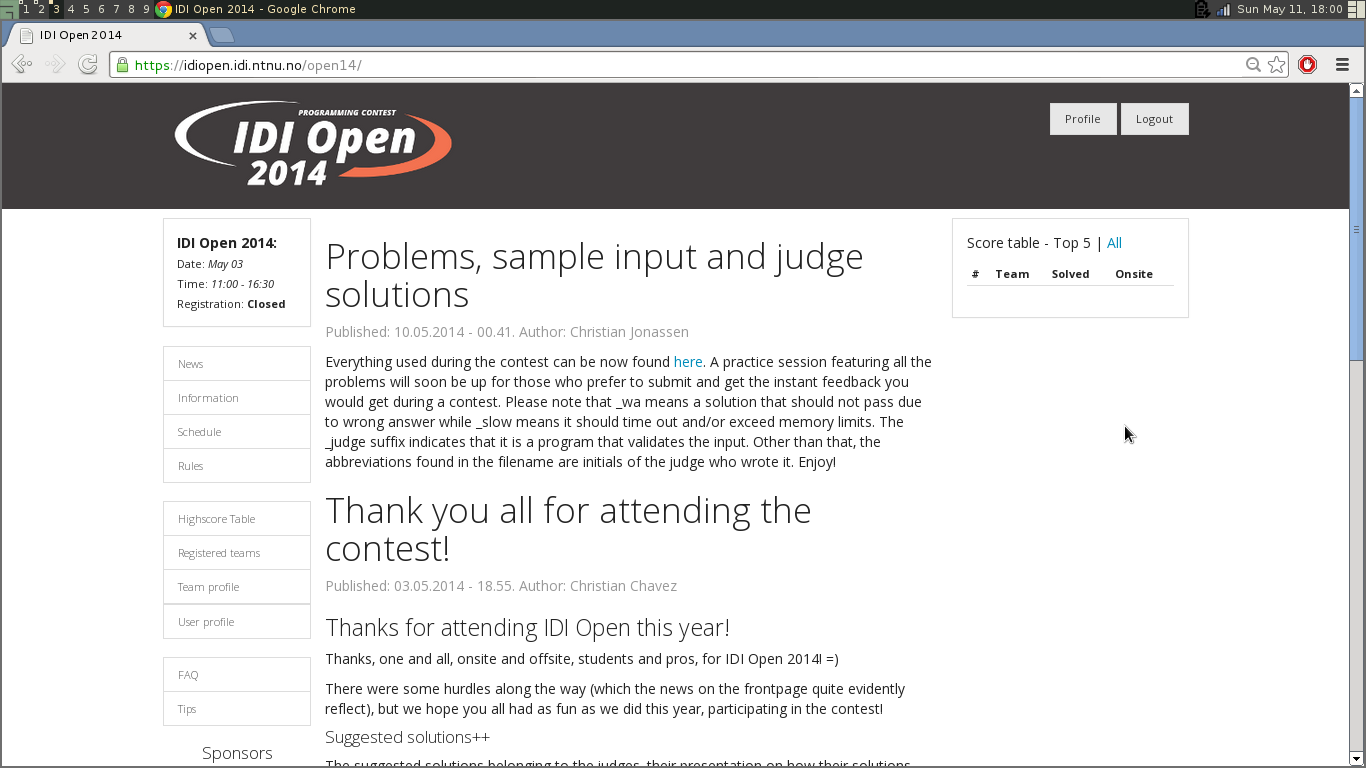
\includegraphics[width=6.4272in,height=3.2602in]{a07Design-img3.png} 
	\caption{Final page}
	\label{fig:finalUI}
\end{figure}

The grey header was in our
initial design coloured blue, but was changed one week before M-07.
This illustrates the strongest
functionality of the design, namely customization. It is possible, by
only uploading a new CSS file, to change the whole feel of the website
and give every contest its own theme. The change from blue to grey was made
as a consequence of IDI Open changing to a new logo. By comparing
Fig~\ref{fig:oldSystem} and Fig~\ref{fig:finalUI}, you can see that we kept the same structure, but
still made some significant changes to the design.


\section{User interface}

The user interface is designed by using a base template. The template is
the same for every part of the webpage, and contains a content block
that changes while you navigate through the different parts. This makes
it easier to add new content to the user interface, because you already
have the base, and don't need to worry about the
header, footer, or the menu. We wanted to make it easy for future
developers to take over GentleIDI after us, and therefore we focused on
a versatile user interface, in case they want to add new functionality.

The menu is placed to the left, coping with the western norm stating
that eye placement is natural to the
left\footnote{\ http://research.microsoft.com/en-us/um/people/cutrell/chi09-buschercutrellmorris-eyetrackingforwebsalience.pdf}.
We designed the menu to be versatile, this was highly prioritized by our customers.
Admins can choose what they want to show in the menu, except for \textit{Register user} and
\textit{Register team} that are ``hardcoded'' on request from the
customer. As mentioned
in Design process ~\ref{sec:designProcess}, we designed the user interface after a principle
of versatility. Admins can also change the logo, the sponsor images and
the contact information in the footer.

Buttons, images and icons were surrounded with boxes, to show that they are different
elements. There is also one big box surrounding a group of elements,
for example the sponsors. This is consistent with the gestalt law of
proximity, that constitutes that humans will naturally group objects
that are close to each other, and view them as distinct.
This helps the user quickly understand the user interface.


 \begin{figure}[h!]
	
\includegraphics[width=2.1807in,height=0.5972in]{a07Design-img4.png} 
	\caption{FIGURECAPTION}
	\label{fig:buttons}
\end{figure}
\begin{figure}[h!]
	
\includegraphics[width=1.0693in,height=0.5in]{a07Design-img5.png} 
	\caption{FIGURECAPTION}
\end{figure}
\begin{figure}[h!]
	
\includegraphics[width=1.1528in,height=0.4028in]{a07Design-img6.png} 
	\caption{FIGURECAPTION}
\end{figure}

``To strive for consistency'' is the
first of Shneiderman's eight golden rules of interface
design\footnote{\ https://www.cs.umd.edu/users/ben/goldenrules.html},
and we tried to follow this while making design decisions. As can be
seen in Fig~\ref{fig:buttons}, we decided to use colours that represents the action
each button is connected to. The red button marks that pressing this
will have permanent consequences. We added a textbox prompt that the
user has to answer after pressing a red button, that constitutes to
Schneiderman's fifth and sixth rule, for easy reversal
of actions and error handling. This wasn't added
initially, but we noticed while testing the system that without a
prompt, it could be possible to leave your team by mistake.
 
\begin{figure}[h!]
	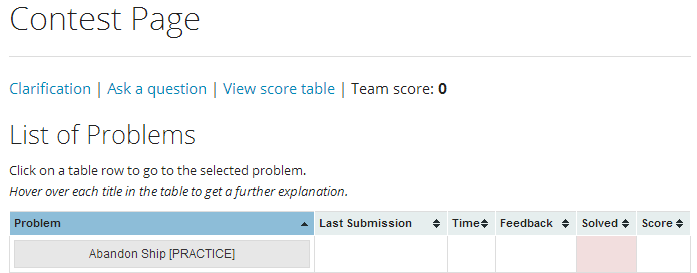
\includegraphics[width=6.5in,height=2.5417in]{a07Design-img7.png} 
	\caption{Contest page}
	\label{fig:contestPage}
\end{figure}

For the contest page, Fig~\ref{fig:contestPage}, we wanted to give the contestant a good
overview of all the problems, their submissions to them, feedback,
if they solved the problem and the score. It is important to not bury
information to deep in a website. It could be challenging to balance
this while trying not to overload the page with too much information.
We had this in mind when designing this page. We got valuable feedback
from the customer concerning what they wanted to be present on the
contest page. They wanted it to be easy for the contestants to access
everything they need during the competition, through the contest page.
After feedback from the customer, we added links to the clarification
page and highscore table on the contest page. This lowers the
short-term memory load on the contestants, which is consistent with
Shneiderman's eight rule, because they will have
everything accessible on the same page.


\section{Admin interface}

 \begin{figure}[h!]
	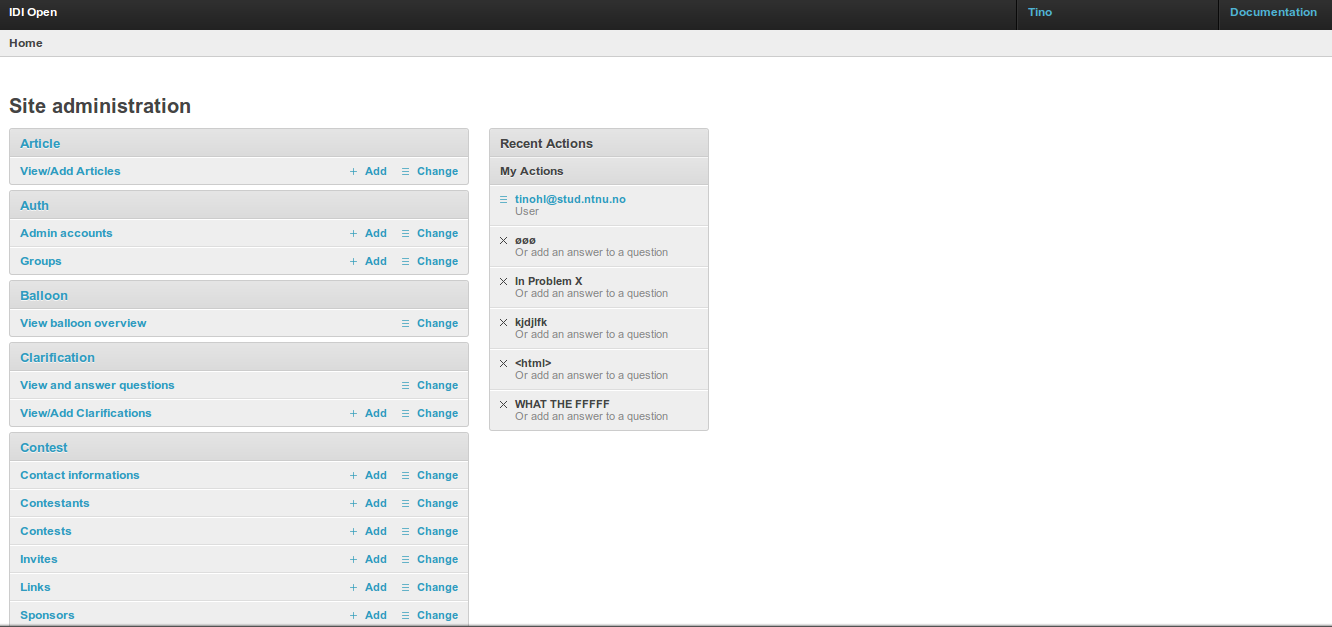
\includegraphics[width=6.5in,height=3.0555in]{a07Design-img8.png} 
	\caption{Admin Interface}
	\label{fig:adminInterface}
\end{figure}

Django comes with an
extensive admin interface, that provides functionality for adding,
removing and changing parts of the system. The interface consists
of everything we as developers want the admins to be able to change.
We decided to use
Grappelli, an app for the django admin interface that also provided us
with more adequate functionality, e.g.\ auto-completion, rich text
editors, drag'n drop and more.

The structure of the layout is simple. Each category has
it's own header and everything in blue is clickable.
The ``Recent Actions'' box is there
to help admins remember what they last did, which is important to
reduce the users short-term memory load, in accordance with
Shneiderman's eight rule.

Originally all the names of the elements were the same as our model
names. We decided to change this to more intuitively understandable
expressions after a request from the customer.
We extended the interface with our own custom views, ``Balloon overview'' and ``Judge views''. 
This allowed us to change 
what we wanted, while it still kept its consistency with the other parts 
of the admin site.



 \begin{figure}[h!]
	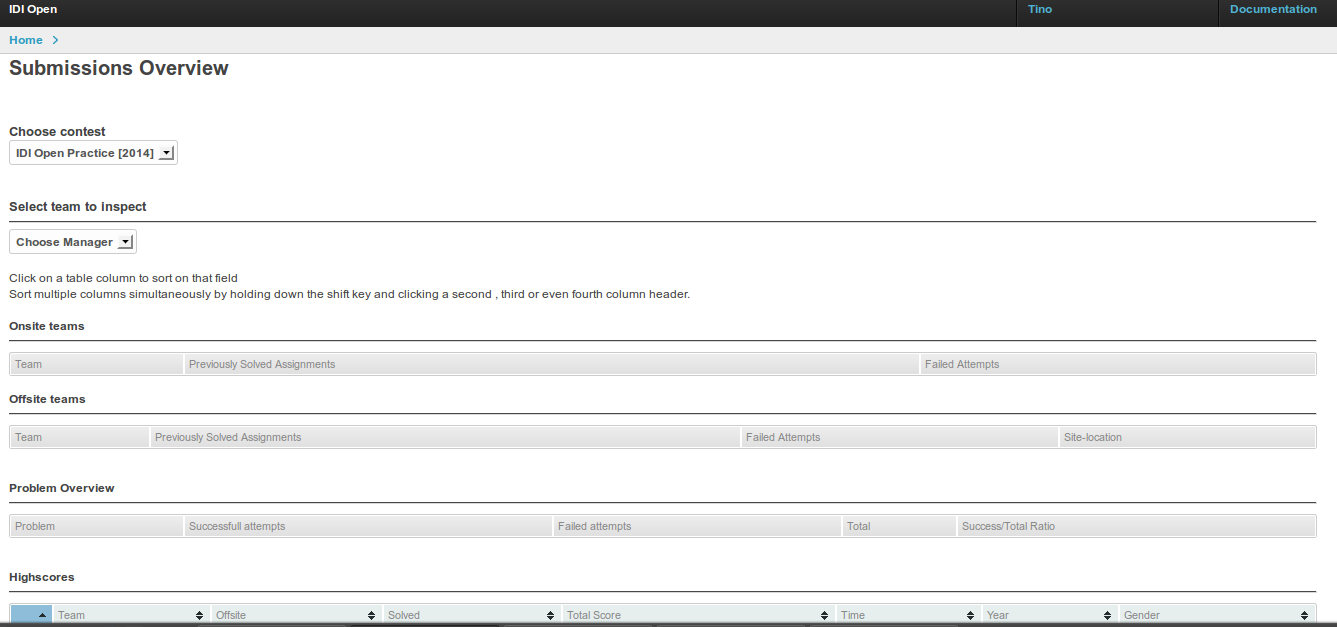
\includegraphics[width=6.5in,height=3.0417in]{a07Design-img9.png} 
	\caption{Judge views}
	\label{fig:judge}
\end{figure}

The judge views was made primarily for judges, but could also be used
by the admins. The motivation behind making this view, is that it gives
the judges a better overview of the competition and how the progress
is going for the different teams. We were initially told that the
judges wanted a way to see if a team was struggling, so they could help
that team. We wanted everything to be on one page for the judges, so they
wouldn't have to constantly switch between different
pages. The judge view can be seen in Fig~\ref{fig:judge}.  

 \begin{figure}[h!]
	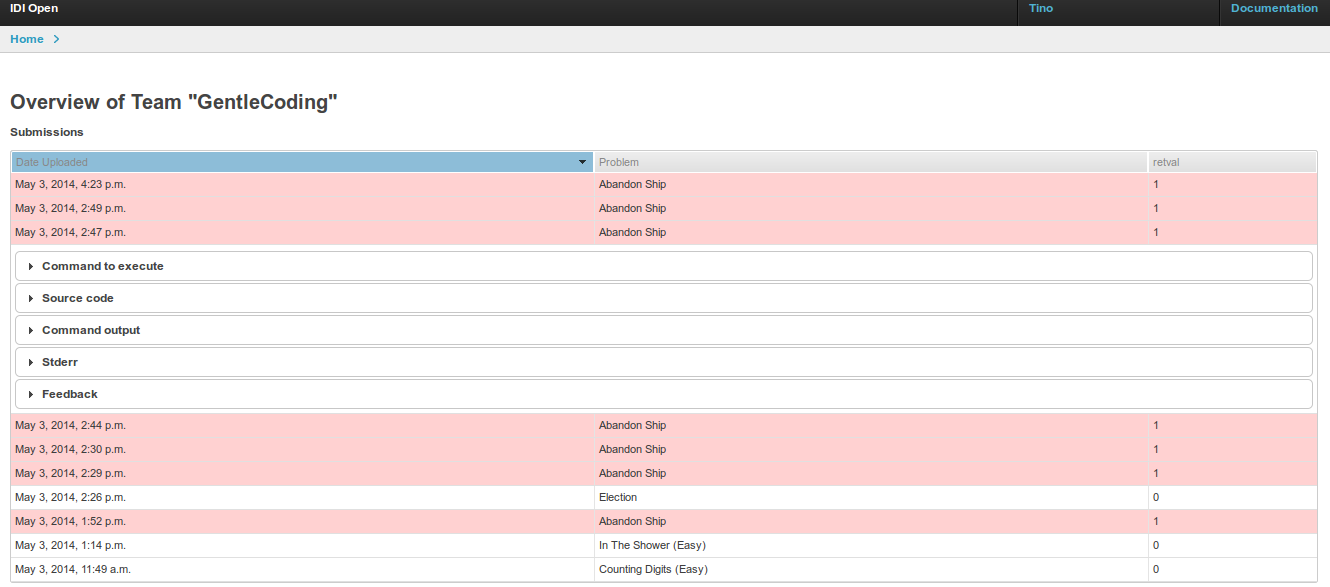
\includegraphics[width=6.5in,height=2.8752in]{a07Design-img10.png} 
	\caption{Judge views for team}
	\label{fig:judgeTeam}
\end{figure}


Fig~\ref{fig:judgeTeam} shows the judge views after
selecting the team ``GentleCoding''.
It is possible to expand each submission by clicking on it. The third
submission has been clicked on, so we can now choose to expand
different categories. For example if a judge wants to see the source
code for that submission, he/she can click on ``Source
code'' and it will expand. Submissions that
haven't been compiled are shown in red, and the other
are white.

\href{http://www.clevelandconsultinggroup.com/articles/emergence-gestalt-approach-to-change.php}
\href{https://www.cs.umd.edu/users/ben/goldenrules.html}
